\documentclass[tikz,border=2mm]{standalone}
\usepackage[utf8]{inputenc} % fixes ä/ö/å etc.
\usepackage[T1]{fontenc}    % better font encoding
\usepackage{tikz}
\usepackage{pgfplots}
\pgfplotsset{compat=1.18}

\begin{document}

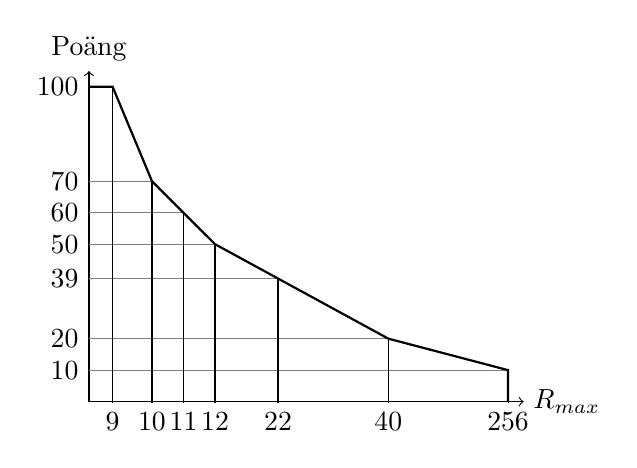
\begin{tikzpicture}[xscale=0.02, yscale=0.04, every node/.style={transform shape=false}]
    \def\xshift{10} % shift everything to the right

    % Draw axes manually
    \draw[->] (0,0) -- (256+\xshift+10,0) node[right] {$R_{max}$}; % x-axis
    \draw[->] (0,0) -- (0,100+5) node[above] {Poäng}; % y-axis

    \coordinate (P1) at (5+\xshift,100);
    \coordinate (P2) at (30+\xshift,70);
    \coordinate (P3) at (70+\xshift,50);
    \coordinate (P4) at (180+\xshift,20);
    \coordinate (P5) at (256+\xshift,10);
    \coordinate (Pmid) at (50+\xshift,60);
    \coordinate (Pmid2) at (110+\xshift,39);
    \coordinate (P0) at (0,0);
    \coordinate (Pneg) at (0,-0.5);

    
    % Draw lines
    \draw[gray, thin] (P1) -- (P1 |- P0);
    \draw[gray, thin] (P2) -- (P2 |- P0);
    \draw[gray, thin] (P3) -- (P3 |- P0);
    \draw[gray, thin] (P4) -- (P4 |- P0);
    \draw[gray, thin] (P5) -- (P5 |- P0);
    \draw[gray, thin] (Pmid) -- (Pmid |- P0);
    \draw[gray, thin] (Pmid2) -- (Pmid2 |- P0);

    \draw[gray, thin] (P2) -- (P0 |- P2);
    \draw[gray, thin] (P3) -- (P0 |- P3);
    \draw[gray, thin] (P4) -- (P0 |- P4);
    \draw[gray, thin] (P5) -- (P0 |- P5);
    \draw[gray, thin] (Pmid) -- (P0 |- Pmid);
    \draw[gray, thin] (Pmid2) -- (P0 |- Pmid2);
    \draw[black, thick] (0,100) -- (P1) -- (P2) -- (P3) -- (P4) -- (P5) -- (256+\xshift,0);


    % x-axis ticks
    \draw (P1) -- (P1 |- Pneg) node[below] {$9$};
    \draw (P2) -- (P2 |- Pneg) node[below] {$10$};
    \draw (Pmid) -- (Pmid |- Pneg) node[below] {$11$};
    \draw (P3) -- (P3 |- Pneg) node[below] {$12$};
    \draw (Pmid2) -- (Pmid2 |- Pneg) node[below] {$22$};
    \draw (P4) -- (P4 |- Pneg) node[below] {$40$};
    \draw (P5) -- (P5 |- Pneg) node[below] {$256$};

    % y-axis ticks
    \draw (-0.5, 100) node[left] {$100$};
    \draw (-0.5, 70) node[left] {$70$};
    \draw (-0.5, 60) node[left] {$60$};
    \draw (-0.5, 50) node[left] {$50$};
    \draw (-0.5, 39) node[left] {$39$};
    \draw (-0.5, 20) node[left] {$20$};
    \draw (-0.5, 10) node[left] {$10$};

\end{tikzpicture}

\end{document}
